\documentclass[oneside,12pt]{book}
\usepackage[utf8]{inputenc}
\usepackage{standalone}
\usepackage[margin=2.5cm]{geometry}
\usepackage{graphicx}
\usepackage{hyperref}
\usepackage{lmodern}
\usepackage{float}
\usepackage{csquotes}
\usepackage[figurename=Ilustración]{caption}
\usepackage[numbers]{natbib}
\usepackage{ragged2e}
\usepackage{array}
\usepackage{multirow}
\usepackage{parskip}
\usepackage{listings}
\usepackage{epigraph}
\usepackage{lipsum} % Texto de relleno en plantilla

\usepackage{comment} %Uso de comentarios multilínea

%\usepackage{fancyhdr}
\usepackage{geometry}
\usepackage{color}\usepackage{graphicx,xcolor}

\usepackage{titlesec}
\setcounter{secnumdepth}{3}
\titleformat{\chapter}[display]
{\normalfont\huge\bfseries}{\chaptertitlename\ \thechapter}{20pt}{\Huge}

\urlstyle{same}
\title{Galería de NFT's en la Web3}
\author{Cristóbal José Jiménez Gómez}
\date{Curso 2022 - 2023}
\renewcommand{\contentsname}{Contenido}
\renewcommand{\figurename}{Ilustración}
\usepackage{pifont}
\renewcommand\labelitemi{\ding{52}}

%Corrección de idioma
\usepackage[spanish,es-tabla]{babel}

%Agregados por mi%
%para la bibliografía%
\usepackage{natbib}
\bibliographystyle{unsrtnat}

%Para las tablas
\usepackage{tabularx}

%Para las imágenes
\usepackage{graphicx}

%Colores 
\usepackage{xcolor}

\begin{document}
\begin{titlepage}
    \begin{center}
    \vspace*{0.5in}
        \begin{figure}[htb]
            \begin{center}
            
\includegraphics[width=15cm]{Ilustraciones/LogoEII.jpg}
            \end{center}
        \end{figure}

        \vspace*{0.15in}
        \vspace*{0.2in}

        \noindent\hfil\rule{11cm}{0.2mm}\hfil\\
        \vspace*{0.1in}
        \begin{Huge}
            \textbf{Galería de NFT's en Web3} \\
        \end{Huge}

        \vspace*{0.3in}

        \begin{large}
            TITULACIÓN: Grado en Ingeniería Informática \\
            \vspace*{0.1in}
            AUTOR: Cristóbal José Jiménez Gómez \\
        \end{large}
        \vspace*{0.3in}
        
        \noindent\hfil\rule{11cm}{0.2mm}\hfil\\

        \vspace*{0.1in}

        \begin{large}
            TUTORIZADO POR: \\
            María Dolores Afonso Suárez \\
        \end{large}
        
    \vspace*{0.3in}

    Fecha: 05/2023
    \end{center}
\end{titlepage}


%\newgeometry{margin=1.5cm}

\thispagestyle{empty}

%\lhead{ 
\begin{tabular}{p{15cm}p{5cm}}
  
\includegraphics{Ilustraciones/LogoEII.jpg}   &  TFT04\\
\end{tabular}
%}

\vspace{1em}
\fboxrule=2pt
\begin{center}
\fcolorbox{gray}{gray!10}{\parbox{.8 \textwidth}{ {\large SOLICITUD DE DEFENSA DE TRABAJO DE FIN DE TÍTULO}}}
\end{center}

\vspace{1em}
\justify
D./Dª Nombre\_Estudiante, autor del trabajo Título\_Trabajo, correspondiente a la titulación Titulación\_Estudiante, en colaboración con la empresa/proyecto Nombre\_Empresa (en su caso)

\vspace{1em}
SOLICITA

\vspace{1em}
que se inicie el procedimiento de defensa del mismo, para lo que se adjunta la documentación requerida, haciendo constar que 

[ ] se autoriza / [ ] no se autoriza la grabación en audio de la exposición y turno de preguntas.

\vspace{1em}
Asimismo, con respecto al registro de la propiedad intelectual/industrial del TFT, declara que:

[ ] Se ha iniciado o hay intención de iniciarlo (defensa no pública).

[ ] No está previsto.

\vspace{1em}
Y para que así conste firma la presente. (fecha en firma electrónica)

\begin{center}
%En Las Palmas de Gran Canaria, a día de mes de año

\vspace{1em}
El/La estudiante

\vspace{3em}
Fdo.------------------------
\end{center}

\begin{center}
\fcolorbox{gray}{white!10}{\parbox{.9\textwidth}{
{\tiny A rellenar y firmar \textbf{obligatoriamente} por el/la/los/las tutores}

En relación con la presente solicitud, se informa:{\tiny (firmar donde corresponda)}

\vspace{1em}
\begin{center}
\begin{tabular}{|p{\dimexpr.45\linewidth}|p{\dimexpr.45\linewidth}|}
%\begin{tabular}{|l|r|}
    \hline
   & \\
  Positivamente {\tiny (en  caso  de  detección  de  copia, esta firma quedará invalidada)}  & Negativamente {\tiny (justificación en TFT05)} \\
   & \\
   & \\
   & \\
   & \\
   & \\
   & \\
  Fdo.------------------------ & Fdo.------------------------  \\
     & \\

    \hline
\end{tabular} 

\end{center}

\vspace{1em}

}
}

\vspace{1em}

%\cfoot{
DIRECTORA DE LA ESCUELA DE INGENIERÍA INFORMÁTICA
%}

\end{center}

\restoregeometry

\clearpage

\newpage
\pagenumbering{arabic}
{\Large{\textbf{Agradecimientos}}}

\begin{flushright}
    {\setlength{\parskip}{8mm}
        \large{
            \textit{A los gnomos de jardín.}
        }
    }
    
\end{flushright}

\clearpage
{\setlength{\parskip}{8mm}
{\huge{\textbf{Resumen}}}

    {\large{ 
        Desarrollo de una Aplicación Web en el marco de la Web3(blockchain), que gestiona una galería de 
        Non Fungible Tokens (NFT’s). Ofrece la gestión de contenidos a distintos tipos de usuarios cuyos niveles de
        interacción varían desde los usuarios sin registrar, a administradores. En esa escala de accesos los
        casos de uso establecerán el nivel de interacción de cada perfil. Las funcionalidades implementadas
        permitirán la gestión a distintos niveles de estos NFT’s, desde la visualización hasta la gestión de cada
        cartera. Este último concepto es el definido para almacenarlos y, en caso de ser necesario comerciar
        (compraventa o intercambio) con ellos.
    }}

    \textbf{Palabras claves:} Web3, Web3.0, Angular, Firebase, Vercel, Express
    

%\newpage

{\huge{\textbf{Abstract}}}

    {\large{
        Development of a Web Application within the framework of Web3 (blockchain), which manages a gallery of
        Non Fungible Tokens (NFT's). It offers content management to different types of users whose levels of
        Interaction range from unregistered users to administrators. At this access scale, the
        use cases will establish the level of interaction of each profile. The functionalities implemented
        will allow the management at different levels of these NFTs, from the visualization to the management of each
        briefcase. This last concept is the one defined to store them and, in case it is necessary to trade
        (purchase or exchange) with them.
    }}

    \textbf{Key Words:} Web3, Web3.0, Angular, Firebase, Vercel, Express
} 
\tableofcontents
\newpage
\listoffigures
\newpage
\listoftables

\clearpage
\pagenumbering{arabic}

%----Introducción----%
%--Motivación/Objetivos/Estructura de memoria--%
\chapter{Introducción}
\section{Motivación}
La razón principal que se encontró para la elaboración de este trabajo ha sido 
el auge de la Blockchain durante estos últimos años. "Blockchain es un libro 
mayor compartido e inalterable que facilita el proceso de registro de 
transacciones y de seguimiento de activos en una red de negocios. Un activo 
puede ser tangible o intangible. Prácticamente cualquier cosa de valor, puede 
rastrearse y comercializarse en una red de blockchain, reduciendo así el 
riesgo y los costes para todos los involucrados"\cite{ibmWeb3}. 

Esta tecnología ofrece la posibilidad de cosntruir aplicaciones web que garanticen
la privacidad y seguridad de los datos de un usuario. La Web 3 ofrece transparencia
y trazabilidad a la hora de la interacción entre usuarios. Además, permite la 
creación o conversión de negocios ya afianzados a este entorno.

Además, se afianza una necesidad que encontraba yo, personalmente, a la hora de
interactuar entre distintas carteras, que es la necesidad de tener todas en una 
misma ubicación.

Se debe constar que ya existen páginas afianzadas para el fin de mostrar y 
compra-venta de NFT's. Este trabajo busca el aprendizaje tanto del desarrollo 
de una aplicación web completa, como de aprender a realizar las llamadas y 
conexiones para recoger y mostrar datos de NFT's\cite{bbcNFTs} y 
criptocarteras\cite{moralisWallets}.

\newpage
\section{Objetivos}
El objetivo principal del proyecto se centra en el desarrollo de un sitio web 
que utiliza el nuevo concepto de descentralización dentro del marco Web3. 
El resultado ofrece como funcionalidad principal la búsqueda de NFT’s y el 
almacenamiento de distintas carteras de criptomonedas. Para ello se plantea 
un conjunto de objetivos generales:
\begin{enumerate}
    \item Estudiar las características y evolución de la Web 3.0 y su relación con la Web3.
    \item Realizar un estudio de las tecnologías y herramientas a emplear.
    \item Establecer criterios para su selección (tanto las tecnologías como de las herramientas)
    \item Seguir una metodología de desarrollo, las pruebas y documentación del proyecto.
\end{enumerate}




\section{Estructura de la memoria}
La memoria está dividida en 10 capítulos diferentes. En ellos se recoge toda
la información, desde el inicio del proyecto hasta las conclusiones. Así, 
la información recogida en cada capítulo se describe tal que:

\-\hspace{1cm} El primer capítulo consta de la introducción al proyecto. En este se 
contextualiza el trabajo, se explica la motivación detrás de la elaboración 
del proyecto, se dan a conocer los objetivos a cumplir y se explica la 
estructura del documento.

\-\hspace{1cm} El segundo capítulo lista y justifica las competencias de la titulación
abarcadas durante el desarrollo del trbajo mediante las teras y actividades realizadas.

\-\hspace{1cm} El tercer capítulo desarrolla el marco teórico, donde se explican y 
analizan algunos términos relevantes a este trabajo. Es el punto de partida, 
donde se realiza una investifación que contextualiza y justifica las cacciones
que se toman en el trabajo.

\-\hspace{1cm} El cuarto capítulo abarca el estado del arte, que explica la 
actualidad del desarrollo Web junto con el desarrollo dentro de la Web3.0 y 
la popularidad entre los distintos frameworks\footnote{Un framework es una 
herramienta de programación que te permite desarrollar software proporcionando 
una estructura con componentes integrados que sirven de base para construir 
proyectos nuevos\cite{bootcampFramework}}

\-\hspace{1cm} El quinto capítulo contiene los recursos y las tecnologías 
utilizadas para el desarrollo del trabajo. En este se definen y justifican.

\-\hspace{1cm} El sexto capítulo se explica la metodología llevada a cabo 
para la realización del trabajo, se dan a conocer als diferentes fases y 
tareas que han existido durante su desarrollo.

\-\hspace{1cm} El séptimo capítulo se incluye un análisis de los requisistos y 
el diseño de la página que se ha elaborado para el desarrollo.

\-\hspace{1cm} El octavo capítulo se explica todo lo relacionado con el 
desarrollo de la página web.

\-\hspace{1cm} El noveno capítulo se encuentra la evaluación de la calidad de la página, 
obtenidos a través de diversos programas o extensiones.

\-\hspace{1cm} El décimo capítulo se incluye las conclusiones que se pueden obtener 
de este proyecto, tanto personales como objetivas, dando además una propuesta de mejora 
para un futuro desarrollo.

\-\hspace{1cm} Finalmente se incluyen los anexos, los cuales también contienen las 
referencias bibliográficas


\newpage
%----Competencias----%
\chapter{Competencias específicas}
Las competencias aplicadas a este proyecto se pueden encontrar en la Tabla 
\ref{tab:competencias} y a continuación se listan: CI8, CI13, CI16, CI17, T12.\\
\-\hspace{1cm} La competencia CI8 se justifica debido a la necesidad de analizar,
diseñar y construir los distintos componentes de la página web, así como las 
estructuras de los distintos documentos de la base de datos.\\
\-\hspace{1cm} La competencia CI13 se justifica por el uso de hacer llamadas a API's
y la creación de un backend. Así como a la hora de desplegar la aplicación a internet. \\
\-\hspace{1cm} La competencia CI16 se justifica debido a la metodología Scrum aplicada
durante el transcurso del proyecto. \\
\-\hspace{1cm} La competencia CI17 se justifica gracias al uso de los programas de 
caldiad utilizados para garantizar la accesibilidad y usabilidad de la página web.\\
\-\hspace{1cm} La competencia T12 se justifica debido a que en eso ha consistido este proyecto: \\
\-\hspace{1.5cm} \textbf{Diseño} de los distintos componentes y páginas de la aplicación.\\
\-\hspace{1.5cm} \textbf{Despliegue} de la aplicación en sus diferentes ramas para poder ser \textbf{evaluadas} 
    por distintos usuarios.\\
\-\hspace{1.5cm} \textbf{Selección} de las herramientas como pueden ser el \textit{framework} sobre el que se ha 
trabajado (Angular), o la página sobre la que se ha hecho el \textit{despliegue}, siempre teniendo en \textit{cuenta el coste 
y la calidad} del mismo.\\

\begin{table}[H]
    \caption{\textbf{Competencias} cubiertas durante el desarrollo del proyecto.}
    \hfill \break
    \label{tab:competencias}
    \begin{tabularx}{\linewidth}{| @{} >{\bfseries}l | >{\RaggedRight}X @{} | }
        \hline
        \centering \textbf{Código} & \textbf{Descripción} \\
        \hline
        CI8  & Capacidad para analizar, diseñar, construir y mantener 
        aplicaciones de forma robusta, segura y eficiente, eligiendo el 
        paradigma y los lenguajes de programación más adecuados. \\ 
        \hline
        CI13 & Conocimiento y aplicación de las herramientas necesarias para el 
        almacenamiento, procesamiento y acceso a los sistemas de 
        información, incluidos los basados en web. \\ 
        \hline
        CI16 & Conocimiento y aplicación de los principios, metodologías y ciclos 
        de vida de la ingeniería del Software \\
        \hline
        CI17 & Capacidad para diseñar y evaluar interfaces persona computador que 
        garanticen la accesibilidad y usabilidad a los sistemas, servicios y 
        aplicaciones informáticas. \\ 
        \hline
        T12  & Capacidad para seleccionar, diseñar, desplegar, integrar, evaluar, 
        construir, gestionar, explotar y mantener las tecnologías 
        de hardware, software y redes, dentro de los parámetros de coste y 
        calidad adecuados.\\ 
        \hline
    \end{tabularx}
    \hfill \break
    \hfill \break
    \centering\textbf{Fuente:} Universidad de Las Palmas de Gran Canaria (2023)
\end{table}
\newpage
%----Estado actual y Objetivos iniciales----%
%--Objetivos iniciales/Estado actual--%
\chapter{Objetivos iniciales y estado actual}
En esta parte del informe se darñan los conceptos generales para la comprensión del mismo.
Se hará un paso por la historia de la Web desde sus inicios hasta como la conocemos ahora 
y se darán los conocimientos básicos para comprender el funcionamiento de las criptomonedas,
los Token's no fungibles y las criptocarteras.
\section{Historia de la Web hasta la Web 3.0}
\label{txt:web3}
La \textbf{World Wide Web} fue creada en 1989 por el científico británico 
\textit{Tim Berners-Lee} mientras trabajaba en el \textit{Centro Europeo de Investigación 
Nuclear(CERN)}. La idea era crear una red de información que pudiera ser compartida 
entre científicos y académicos de todo el mundo. Para evitar un apagado accidental se escribió 
una nota en tinta roja (Figura \ref*{fig:cern-server}) que ponía: "\textcolor{red}{This machine is a server. DO NOT 
POWER IT DOWN!!}"\cite{cernWeb1} (Esta máquina es un servidor. ¡¡NO LO APAGUEN!!) \\
\begin{figure}[htb!]
    \caption{Pegatina del servidor del CERN con la WWW}
    \label{fig:cern-server}
    \centering
    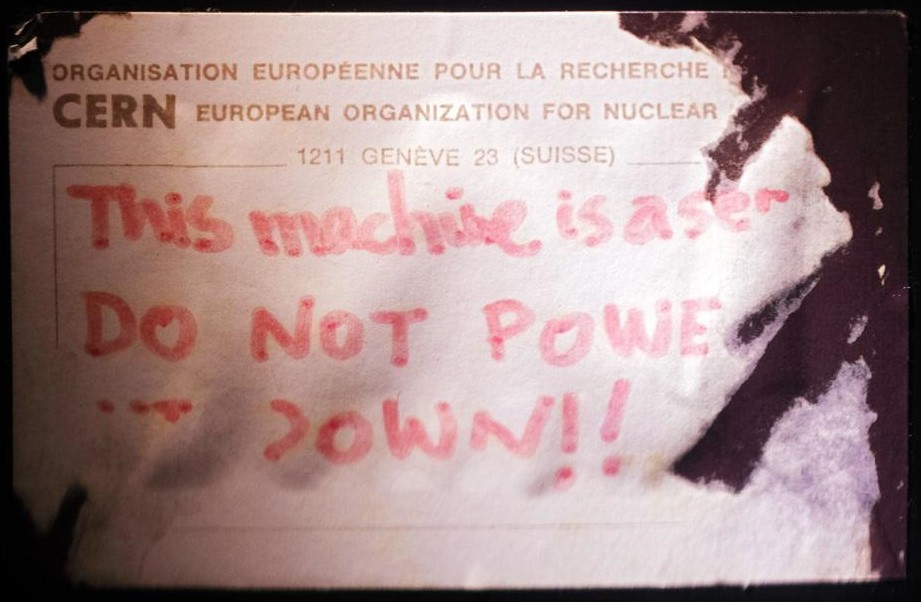
\includegraphics[scale=0.25]{./Ilustraciones/cern-server.jpg}\\
    \textbf{Fuente:} Reddint oficial del CERN [\url{https://www.reddit.com/r/CERN/}]
\end{figure}


\hfill \break
In 1991, \textit{Berners-Lee} creó una serie de tecnologías que permitían la 
conexión de documentos en un sistema hipertextual, utilizando el 
\textit{protocolo \textbf{HTTP}} y la \textit{codificación \textbf{HTML}}. 
Esto permitió a los usuarios navegar por la red y acceder a documentos 
enlazados desde cualquier parte del mundo. \\
\hfill \break
Con el tiempo, la Web se expandió y evolucionó, surgieron nuevas tecnologías como los 
motores de búsqueda, las redes sociales y las aplicaciones móviles, lo que llevó
a la denominada \textbf{Web 2.0}.\\
\hfill \break
La Web 2 se caracterizó por una mayor interactividad, el desarrollo de 
aplicaciones colaborativas y la creación de plataformas para la participación 
del usuario, como blogs, wikis y redes sociales. La Web2 también permitió la 
creación de empresas en línea y el desarrollo de nuevos modelos de negocio basados 
en la publicidad y los servicios en línea.\cite{web2Explained}\\
\hfill \break
La \textbf{Web 3}, también conocida como \textit{Web descentralizada}, 
es la siguiente evolución de la Web. La Web 3.0 se centra en la descentralización 
de la web, lo que significa que los usuarios tienen mayor control sobre sus 
datos y pueden interactuar directamente entre sí sin la necesidad de 
intermediarios centralizados.\\
\hfill \break
La tecnología clave detrás de la Web 3 es la cadena de bloques (blockchain) y 
otras tecnologías de registro distribuido (DLT), que permiten la creación de 
aplicaciones descentralizadas (dApps) y contratos inteligentes (smart contracts). 
Esto permite la creación de aplicaciones que no estén sujetas a la censura, la 
interferencia o la dependencia de un solo proveedor, lo que a su vez ofrece 
mayor privacidad y seguridad para los usuarios.\\
\hfill \break
En resumen, la Web ha evolucionado desde su creación como WWW hasta la 
actualidad de la Web3. La Web 3 representa una evolución hacia un internet 
más descentralizado y democrático, donde los usuarios tienen un mayor control 
sobre sus datos y su experiencia en línea, y donde la confianza y la seguridad 
se pueden garantizar a través de la tecnología blockchain y otros mecanismos 
de confianza descentralizados.\cite{IEEEweb3Explained}\\
\section{Concepto de Cryptomoneda}
\label{txt:criptomoneda}
Las \textbf{criptomonedas} son monedas digitales que utilizan tecnología 
criptográfica para asegurar y verificar las transacciones y para controlar 
la creación de nuevas unidades de la moneda. Las criptomonedas funcionan en una 
red descentralizada, lo que significa que no están controladas por ningún 
gobierno, banco central o entidad financiera.\\
\hfill \break
Cada criptomoneda tiene su propia \textbf{red de blockchain} (Figura \ref*{fig:redes}), 
que es un registro público descentralizado que registra todas las transacciones 
de la moneda. La blockchain es una base de datos distribuida que contiene 
todas las transacciones realizadas con la moneda desde su creación, y se 
utiliza para verificar y validar las transacciones y para asegurar que no 
se puedan crear unidades adicionales de la moneda sin cumplir ciertas 
condiciones.\\
\hfill \break
\begin{figure}[htb!]
    \caption{Las redes más populares según Metamask}
    \label{fig:redes}
    \centering
    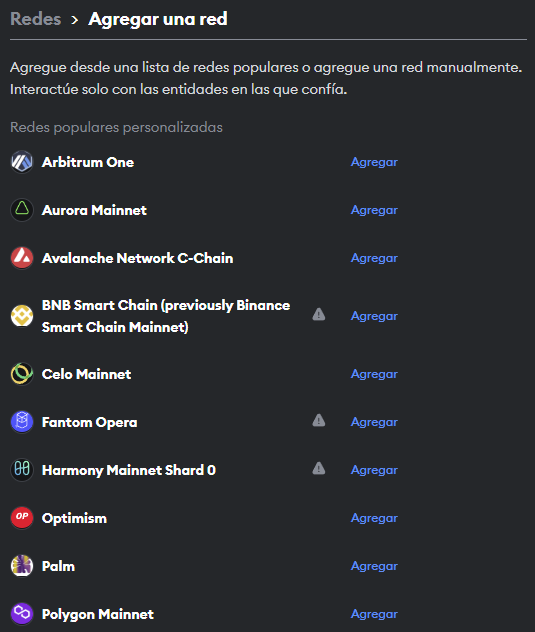
\includegraphics[scale=0.75]{./Ilustraciones/redes.png}\\
    \textbf{Fuente:} Cuenta personal de Metamask al querer agregar una nueva red a día 04/05/2023
\end{figure}
\hfill \break
Las \textbf{transacciones} en una criptomoneda se realizan de forma peer-to-peer (entre 
pares) y se validan a través de un proceso llamado \textbf{minería}. Esta es 
un proceso mediante el cual los usuarios de la red utilizan su poder
de cómputo para resolver problemas matemáticos complejos y validar las 
transacciones en la blockchain. Los usuarios que realizan esta tarea reciben 
recompensas en forma de nuevas unidades de la criptomoneda.\\
\hfill \break
Las criptomonedas se pueden comprar y vender en plataformas de intercambio de 
criptomonedas, y su valor depende de la oferta y la demanda del mercado.\\ 
\hfill \break
Ofrecen varias ventajas, como la descentralización, la transparencia, la 
seguridad y la privacidad, pero también presentan algunos desafíos, como la 
volatilidad del valor y la falta de regulación.\\
\hfill \break
En resumen, las criptomonedas son monedas digitales que utilizan tecnología 
criptográfica y una red descentralizada para asegurar y verificar las 
transacciones. Las criptomonedas se pueden comprar y vender en plataformas de 
intercambio, y su valor depende de la oferta y la demanda del mercado. Las 
criptomonedas como todo en la vida, tiene sus ventajas y sus riesgos.\\
\section{Concepto de NFT}
\label{txt:nft}
Los \textbf{tokens no fungibles} (\textbf{NFT}, por sus siglas en inglés) son 
activos digitales únicos que se utilizan para representar elementos digitales 
como obras de arte, videos, música, juegos, entre otros. A diferencia de las 
criptomonedas tradicionales, los NFT no son intercambiables y cada uno es 
único e irrepetible.\\
\hfill \break
Los NFT se basan en la \textbf{tecnología blockchain} y utilizan contratos 
inteligentes (\textbf{smart contracts}) para garantizar la propiedad y 
autenticidad del activo digital que representan. Los contratos inteligentes 
se utilizan para definir las condiciones y términos de la transacción, y 
garantizan que solo el propietario del NFT tenga derecho a la propiedad del 
elemento digital que representa.\\
\hfill \break
Los NFT se han vuelto muy populares en el mundo del arte digital, ya que 
permiten a los artistas vender sus obras de arte como activos únicos[ 
Por ejemplo, la figura \ref*{fig:opensea-nft}] y garantizar su 
autenticidad y propiedad. También se están utilizando en otros sectores como 
los videojuegos, donde se pueden utilizar para representar objetos y personajes 
únicos [Por ejemplo, la figura \ref*{fig:sorare-nft}].\\
\hfill \break
\begin{figure}[htb!]
    \caption{Muestra de algunos NFT's de la collección de Moonbirds}
    \label{fig:opensea-nft}
    \centering
    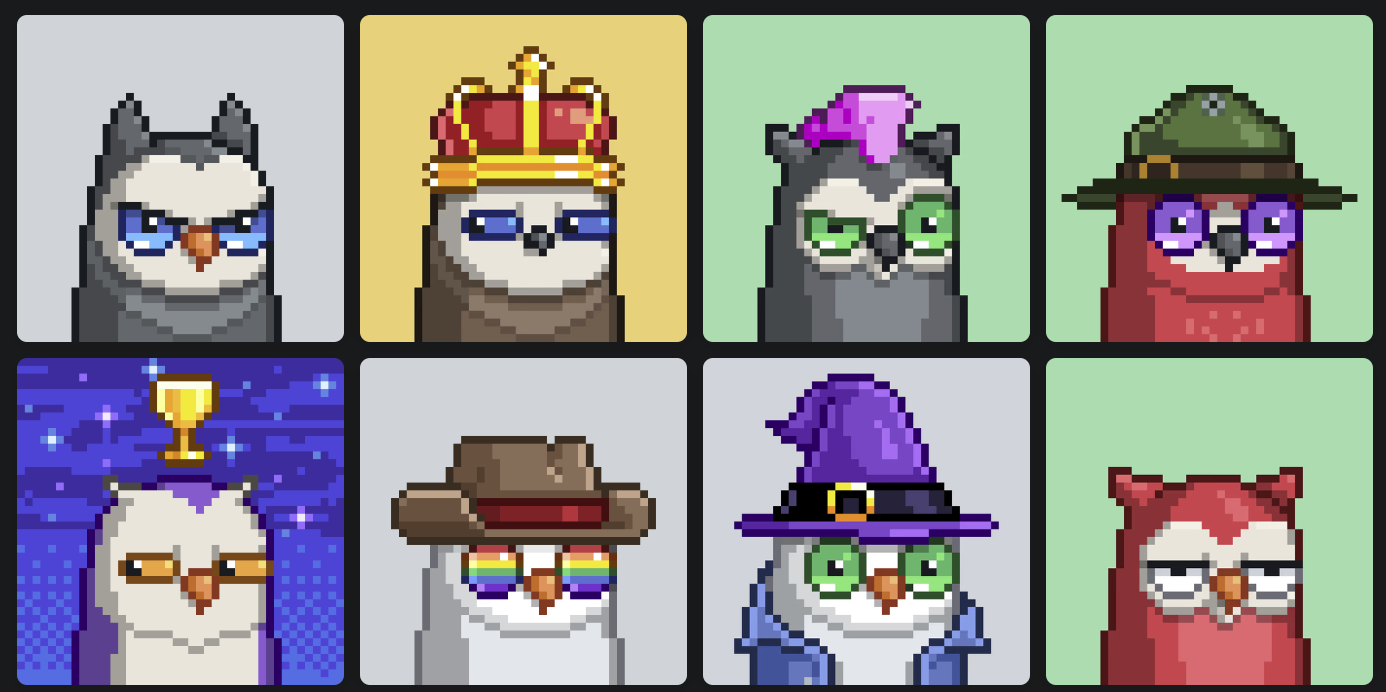
\includegraphics[scale=0.25]{./Ilustraciones/opensea-nft.png}\\
    \textbf{Fuente:} Página de OpenSea [\url{https://opensea.io}]- Collección Moonbirds a día 03/04/2023
\end{figure}
\hfill \break
\begin{figure}[htb!]
    \caption{Muestra de algunos NFT's de la Sorare}
    \label{fig:sorare-nft}
    \centering
    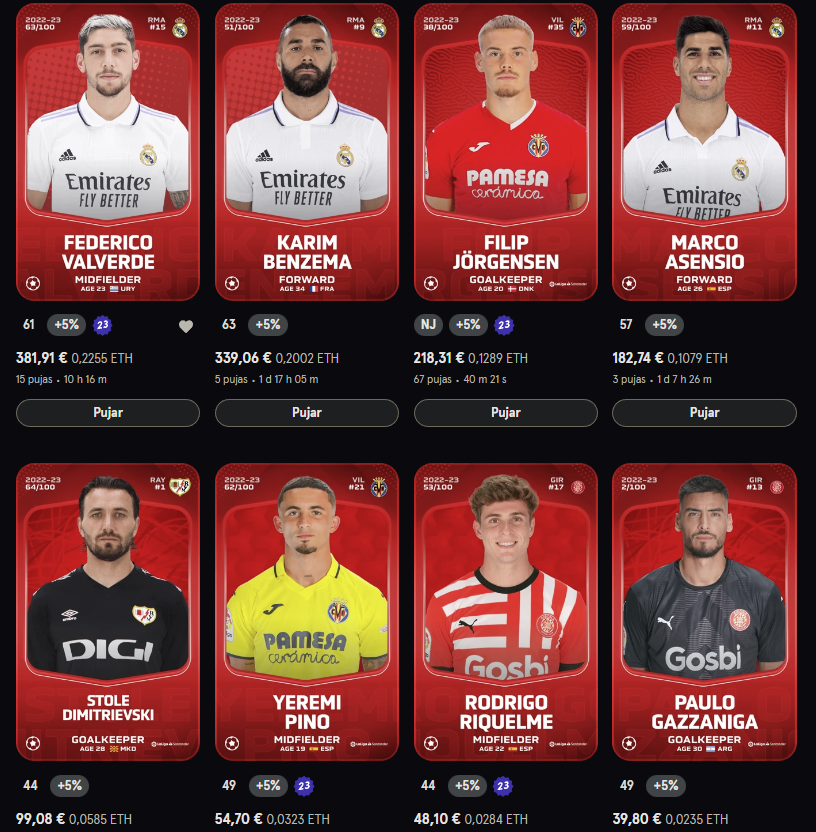
\includegraphics[scale=0.5]{./Ilustraciones/sorare-nft.png}\\
    \textbf{Fuente:} Página de Sorare [\url{https://sorare.com/}]- Sección de mercado con 
    filtros de jugador raro de la Liga Santander a día 03/04/2023
\end{figure}
El valor de un NFT depende de la demanda del mercado y de la percepción del 
valor del activo digital que representa. Los NFT se pueden vender y comprar 
en plataformas especializadas y se utilizan principalmente como activos de 
inversión o de colección.\\
\hfill \break
En resumen, los NFT son activos digitales únicos que se utilizan para 
representar elementos digitales como obras de arte, videos, música, juegos, 
entre otros, y se basan en la tecnología blockchain y contratos inteligentes 
para garantizar la propiedad y autenticidad del activo digital que representan. 
Los NFT se han vuelto muy populares en el mundo del arte digital y se están 
utilizando en otros sectores como los videojuegos\cite{xatakaNFT}.\\
\hfill \break
\newpage
\section{Concepto de CryptoCartera}
\label{txt:wallet}
Una \textbf{criptocartera} es una herramienta que se utiliza para almacenar, 
enviar y recibir criptomonedas. Es similar a una billetera física, pero en 
lugar de contener billetes y monedas, una criptocartera contiene claves 
privadas y públicas que permiten acceder y administrar las criptomonedas.\\
\hfill \break
Cada criptomoneda tiene su propia criptocartera, y hay varios tipos de 
criptocarteras disponibles, incluyendo carteras de hardware, software y en 
línea. Las \textbf{carteras de hardware} (Figura \ref*{fig:ledger}) son dispositivos físicos que se conectan a 
un ordenador y se utilizan para almacenar las claves privadas de manera segura. 
Las \textbf{carteras de software} se descargan en un ordenador o dispositivo 
móvil y se utilizan para almacenar las claves privadas en un archivo cifrado. 
Las \textbf{carteras en línea}(Figura \ref*{fig:coinbase}) se almacenan en la nube y se pueden acceder 
desde cualquier dispositivo con una conexión a internet.
\begin{figure}[htb!]
    \caption{Criptocartera Hardware}
    \centering
    \label{fig:ledger}
    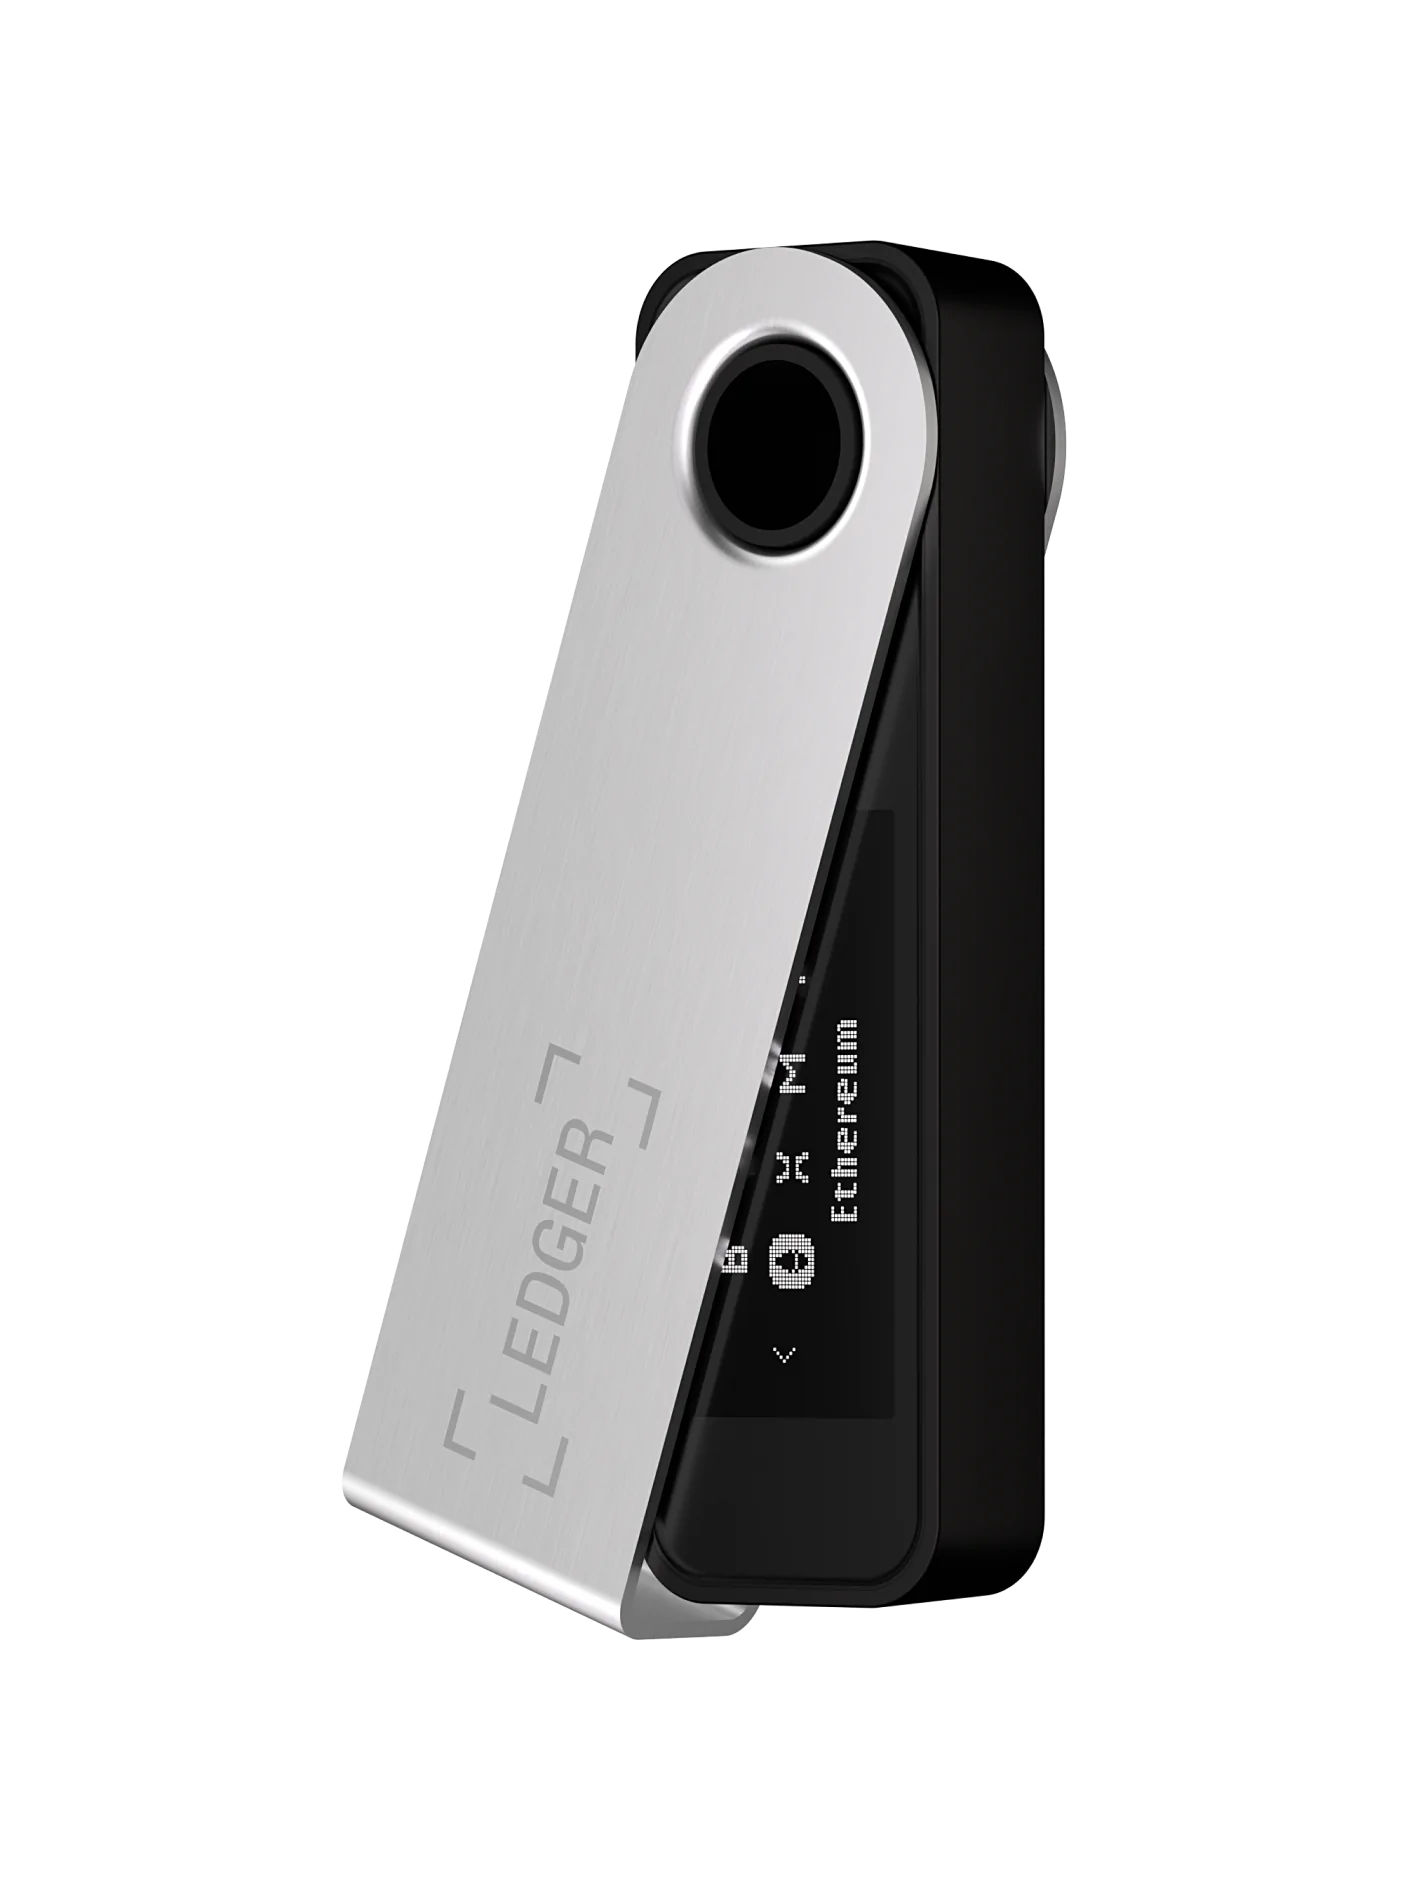
\includegraphics[scale=0.15]{./Ilustraciones/ledger-hardware.png}\\
    \textbf{Fuente:} Página oficial de Ledger [\url{https://shop.ledger.com/products/ledger-nano-s-plus}]
\end{figure}
\hfill \break
\begin{figure}[htb!]
    \caption{Criptocartera Online}
    \label{fig:coinbase}
    \centering
    
\includegraphics[scale=1]{./Ilustraciones/coinbase-logo.png}\\
    \textbf{Fuente:} Logo oficial de Coinbase  [https://www.coinbase.com/es/]
\end{figure}
Las criptocarteras son importantes porque las criptomonedas no se almacenan en 
un lugar centralizado, como un banco, sino que se almacenan en la blockchain de 
la criptomoneda. Por lo tanto, es necesario utilizar una criptocartera para 
acceder y administrar las criptomonedas.\\
\hfill \break
Las criptocarteras también permiten \textbf{enviar y recibir criptomonedas}
de forma segura. Para enviar criptomonedas, se necesita la dirección pública 
de la criptocartera del destinatario. Para recibir criptomonedas, se proporciona 
la dirección pública de la criptocartera al remitente.\\
\hfill \break
En resumen, una criptocartera es una herramienta utilizada para almacenar, 
enviar y recibir criptomonedas. Hay varios tipos de criptocarteras disponibles, 
incluyendo carteras de hardware, software y en línea. Las criptocarteras son 
importantes porque permiten acceder y administrar las criptomonedas, que se 
almacenan en la blockchain de la criptomoneda.
\newpage
%----Desarrollo como concepto----%
\begin{comment}
        CAPÍTULO OBLIGATORIO
        Metodología aplicada y desarrollo del trabajo en sus distintas fases, decisiones de diseño, herramientas empleadas.
        Si el trabajo incluye software desarrollado, deberán seleccionarse las secciones más relevantes del mismo y comentarlas en la memoria.
        Ajuste a la planificación inicialmente prevista.
        Modificación en los objetivos planteados.
\end{comment}
\chapter{Marco teórico}
\newpage
\chapter{Recursos y tecnologías}
\newpage
\chapter{Metodologías}
\newpage
\chapter{Análisis y Diseño}
\newpage
\chapter{Desarrollo}
\newpage
%----Fin del Desarrollo----%

%----Evaluación y resultados----%
\chapter{Evaluación y resultados}

%----Conclusiones y trabajo futuro----%

\chapter{Conclusiones y trabajo futuro}
%\input{Conclusiones.tex}
CAPÍTULO OBLIGATORIO

Resultados,  grado  de  consecución  de  los  objetivos,  posibles extensiones
\newpage

\bibliography{bib.bib}

\end{document}